\documentclass[11pt]{article}\usepackage[]{graphicx}\usepackage[]{color}
% maxwidth is the original width if it is less than linewidth
% otherwise use linewidth (to make sure the graphics do not exceed the margin)
\makeatletter
\def\maxwidth{ %
  \ifdim\Gin@nat@width>\linewidth
    \linewidth
  \else
    \Gin@nat@width
  \fi
}
\makeatother

\definecolor{fgcolor}{rgb}{0.345, 0.345, 0.345}
\newcommand{\hlnum}[1]{\textcolor[rgb]{0.686,0.059,0.569}{#1}}%
\newcommand{\hlstr}[1]{\textcolor[rgb]{0.192,0.494,0.8}{#1}}%
\newcommand{\hlcom}[1]{\textcolor[rgb]{0.678,0.584,0.686}{\textit{#1}}}%
\newcommand{\hlopt}[1]{\textcolor[rgb]{0,0,0}{#1}}%
\newcommand{\hlstd}[1]{\textcolor[rgb]{0.345,0.345,0.345}{#1}}%
\newcommand{\hlkwa}[1]{\textcolor[rgb]{0.161,0.373,0.58}{\textbf{#1}}}%
\newcommand{\hlkwb}[1]{\textcolor[rgb]{0.69,0.353,0.396}{#1}}%
\newcommand{\hlkwc}[1]{\textcolor[rgb]{0.333,0.667,0.333}{#1}}%
\newcommand{\hlkwd}[1]{\textcolor[rgb]{0.737,0.353,0.396}{\textbf{#1}}}%
\let\hlipl\hlkwb

\usepackage{framed}
\makeatletter
\newenvironment{kframe}{%
 \def\at@end@of@kframe{}%
 \ifinner\ifhmode%
  \def\at@end@of@kframe{\end{minipage}}%
  \begin{minipage}{\columnwidth}%
 \fi\fi%
 \def\FrameCommand##1{\hskip\@totalleftmargin \hskip-\fboxsep
 \colorbox{shadecolor}{##1}\hskip-\fboxsep
     % There is no \\@totalrightmargin, so:
     \hskip-\linewidth \hskip-\@totalleftmargin \hskip\columnwidth}%
 \MakeFramed {\advance\hsize-\width
   \@totalleftmargin\z@ \linewidth\hsize
   \@setminipage}}%
 {\par\unskip\endMakeFramed%
 \at@end@of@kframe}
\makeatother

\definecolor{shadecolor}{rgb}{.97, .97, .97}
\definecolor{messagecolor}{rgb}{0, 0, 0}
\definecolor{warningcolor}{rgb}{1, 0, 1}
\definecolor{errorcolor}{rgb}{1, 0, 0}
\newenvironment{knitrout}{}{} % an empty environment to be redefined in TeX

\usepackage{alltt}

\usepackage{rotating}
\usepackage{graphics}
\usepackage{latexsym}
\usepackage{color}
\usepackage{listings}
\usepackage{wrapfig}
\usepackage{float}
\usepackage[belowskip=-15pt,aboveskip=0pt]{caption}

\setlength\topmargin{-.56in}
\setlength\evensidemargin{0in}
\setlength\oddsidemargin{0in}
\setlength\textwidth{6.49in}
\setlength\textheight{8.6in}
\setlength{\intextsep}{10pt plus 1pt minus 4pt}

\definecolor{codegreen}{rgb}{0,0.6,0}
\definecolor{codegray}{rgb}{0.5,0.5,0.5}
\definecolor{codepurple}{rgb}{0.58,0,0.82}
\definecolor{backcolour}{rgb}{0.95,0.95,0.92}
\lstdefinestyle{mystyle}{
	backgroundcolor=\color{backcolour},   
	commentstyle=\color{codegreen},
	keywordstyle=\color{magenta},
	numberstyle=\tiny\color{codegray},
	stringstyle=\color{codepurple},
	basicstyle=\footnotesize,
	breakatwhitespace=false,         
	breaklines=true,                 
	captionpos=b,                    
	keepspaces=true,                 
	numbers=left,                    
	numbersep=5pt,                  
	showspaces=false,                
	showstringspaces=false,
	showtabs=false,                  
	tabsize=2
}
\lstset{style=mystyle}

\pagestyle{headings}

\title{Tumor Penetration Rates for Prostate Cancer\vspace{-5ex}} 
\date{November 12, 2020\vspace{-5ex}}
\IfFileExists{upquote.sty}{\usepackage{upquote}}{}
\begin{document} 
\maketitle
\hfill \break


















\noindent\textbf{\underline{Executive Summary}}: With the common prostate canceri diagnostic among men, the goal of this analysis is to find the variable that could predict the chances of a tumor has penetrated the prostatic capsule. A dataset was provided by the Ohio State University Comprehensive Cancer Center to analyze how demographic and screening results could cause the likelihood of penetration. A tool was built using multiple logistic regression to predict the chances of a patients getting diagnosed with prostate cancer using three variables results of digital rectal exam, Prostatic Specific Antigen value, and total Gleason score. This model was proved to be the best model with an AUC of 0.82, an accuracy of 0.77, Sensitivity of .75, and Specificity of .79. Some interesting findings includes a 269\% increase in chances of having prostate cancer when a patient has a unilobar nodule from the left on their results of digits rectal exam compared to patient with no nodule. Furthermore, patients who has bilobar nodule results after their digital rectal exam will have higher chance of having prostate cancer compared to patient with no nodule, 260\% more to be exact. In addition, patients could gain 133\% more likelihood of being diagnosed with prostate cancer when they have a higher Gleason score. Knowing these three variables (results of digital rectal exam, Prostatic Specific Antigen value, and total Gleason score) are significant factor of the likelihood of penetration rate in protate cancer, health care professionals would be more cautious in treating each patients. In addition, patients could detect their prostate cancer stages earlier and seek help accordingly.      
\hfill \break

\noindent\textbf{\underline{Introduction}}: Prostate cancer is one of the most common cancers among men. The survival rate is vary depending on the stages of the cancer. Prostate cancer has a high probability of being treated if detected at early stages. There are many important characteristics that can predict whether a tumor has penetrated the prostatic capsule. With the results of penetration rate, doctors and nurses would prioritize the patients with the high risk level. On the other hand, if the patients have low rate in penetration, health care workers could find the best treatments for them to slow down prostate growth rate or even treat the patients. With this being said, hostpitals can plan their budget and supplies to focus more on high risk patients and minimize supplies to low risk patients. Knowing penetration rates does not only benefits doctors and nurses, it would also help all men out there to detect if their tumors have penetrated the prostatic capsule. This way, patients would seek professional help at an earlier stage to increase their survival rate. Many questions have proposed in favor of these issues including 1) What variables cause the penetration rate to increase or decrease? 2) What are the likelyhood of penetration rate? 3) How accruate is the model proposed in this analysis? 4) How can we implement the model for everyone to use? and 5) How can we improve the current model? This report will answer all of the questions mentioned above by crucials data analysis process such as data exploratory analysis process to explore the relationship of each variables, model development using multiple logistic regression to built model, and diagnositics process to check the quality of the model. This model will serve the purpose of predicting penetration rate for prostate cancer in men to minimize human errors and provide an effective tool for health care workers.
\hfill \break

\noindent\textbf{\underline{Methods}}: A subset of data was provided from the Ohio State University Comprehensive Cancer Center to find the variables to predict if a tumor has penetrated the prostatic capsule. This data set contain a total of 380 subjects, out of which, 153 subjects had a cancer that penetrated the capsule. There are three observations contain missing values. After eleminating missing values to build more quality models, the dataset now have a total of 377 observations. These data contains one identification column with numbers of each subject, two demographic columns including age and race of the subjects, and four health measurements such as the results of digital rectal exam, detection of capsular involvement, prostatic specific antigen value, and total gleason score. Health mesurement variables will be explained in details in the exploretory data analysis section. The goal of this analysis is to find the average tumor penetration of prostatic capsule rate. To accomplish this goal, we will first analyze the relationship between each predictor and target variable, build models using bootstraping method, consider interaction terms to be in the final model, check for the quality of the models, and conclude with an interpretaion of the model output. All analysis will be done in R Studio with R version 3.6.2.        
\hfill \break

\noindent\textbf{\underline{Exploratory Data Analysis}}: Before picking variables for our model development procress, it is important to access the relationship of each response variable with the target variable. Table~A\ref{descrips} shows an descriptive statistics of each independent variable. As seen in this table, the maximum value of Prostatic Specific Antigen value are relatively high compare to the median and mean values suggesting there might be outliers. In addition, there are disproportion weights of each factor in race of the subjects and detection of capsular involvement. This indicates that there might be biased in predicting the outcome if we use these two variables in the models. The rest of the variables seems proportionally balanced and no skewness were detected among them. In terms of the tumor penetration of prostatic capsule, the response variable has a balance proportion of 40\% of tumor has penetrated the prostatic capsule out of 377 subjects. Figure~\ref{explore1}.1 show the histogram of chances of the tumor penetration of prostatic capsule (1 = penetration, 0 = no penetration).  

\begin{figure}[h!] 
\begin{center}

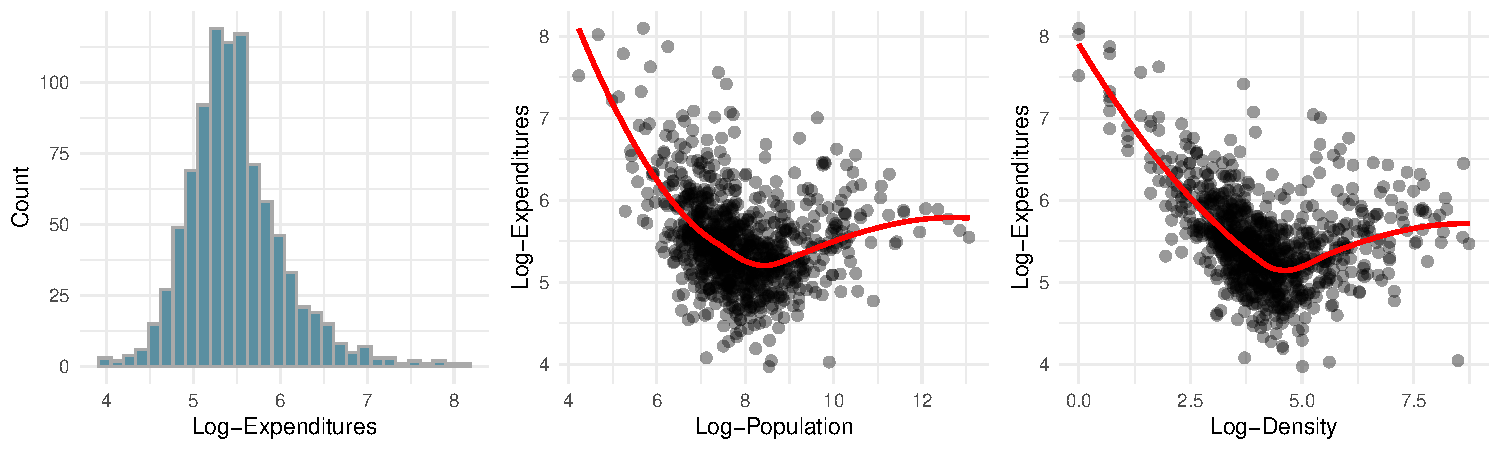
\includegraphics[width=\maxwidth]{figure/unnamed-chunk-1-1} 

\caption{Histogram of 1 (Left): Tumor Penetration of prostatic capsule (1 = penetration) and 2 (Right): Results of Digital Rectal Exam (1 = no nodule, 2 = unilobar nodule left, 3 = unilobar nodule right, 4 = bilobar nodule) with average penetration rate in black.}
\label{explore1}
\end{center} 
\end{figure}

\noindent The results of digital rectal exam is a simple exam to check the prostate to determine the size of the prostate and any abnormalities. Clearly, different abnormalities would have different chances of penetration of prostatic capsule. Figure~\ref{explore1}.2 shows four categories of the results of digital rectal exam including no nodule, unilobar nodule (left), unilobar nodule (right), and bilobar nodule noting using number from 1 to 4, respectively. Here, this variable is identified as categorical variables with four levels instead of a continuous variable. As seen in plot, these four categories obviously have different average penetration rates. For example, a subject with no nodule would be less likely to penetrate compare to a person with bilobar nodule. It makes sense because if there is no nodule detected in the prostate area, then there is less chances of the tumor will penetrate the prostatic capsule. In addition, Figure~\ref{explore1}.2 also depicts the number of subject in each category. Unilobar nodule (left) is the most common and bilobar nodule is the least common among prostate cancer. However, the proportion of each factor for digital rectal exam are not too different. Thus, this variables would provide significant impact for the models.   
\hfill \break

\noindent Detection of capsular involvement can describe if the tumor involving or extending beying the prostate capsule. The tumor is involved when there is capsular involment present. Clearly, the patients who have capsular involement present can be more risky than patient who do not have capsular involment. Figure~\ref{explore2}.1 shows the count and proportion of penetration for the detection of capsular involement. This variable has two levels (1 = no, 2 = yes) to suggest if a subject has capsular involvement or not. As seen in the figure, patients with capsule involement would be much more likely to have tumor penetrated of prostatic capsule compare to patients that do not have capsule involvement. However, the count for each level is not proportional. The majority of the subject have level 1, no capsular involement. Therefore, this variable could be a good variable for our model since it shows a strong signal, however, cautious about the disproportional need to be consider before finalizing the model.      

\begin{figure}[h!] 
\begin{center}

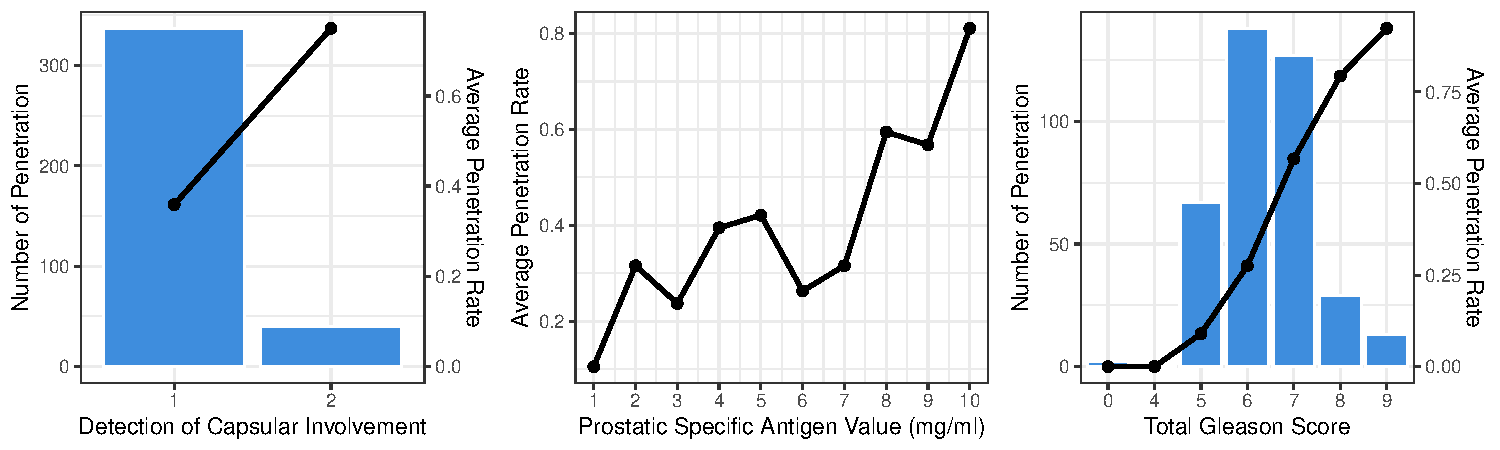
\includegraphics[width=\maxwidth]{figure/unnamed-chunk-2-1} 

\caption{Plots of each variable with average penetation rate in black of 1 (Left): Dectation of capsular involvement along with the frequency of each factor, 2 (Center): Prostatic Specific Antigen value with mg/ml unit by decile, and 3 (Right): Total Gleason score along with its histogram.}
\label{explore2}
\end{center} 
\end{figure}

Prostatic Specific Antigen (PSA) can be found in the prostate gland cells. This screening test measure the amount of prostate-specific antigen in patients' blood using miligram per mililitter (mg/ml). Higher PSA level could lead to a high posibility of diagnosting with prostate cancer. Figure~\ref{explore2}.2 show a plot of the relationship between PSA and the average penetration of prostatic capsule rate. Here, the data point is being sorted from smallest to highest, divided into 10 equal buckets, and assinged a decide for visualization purposes. As on can see, as the decile number increases by one unit, the chances of penetration rate increases, on average. Since PSA in higher buckets are generally the largest, they have higher risk of getting prostate cancer than PSA in lower buckets. Therefore, this proves that PSA could provide signicant relationship for the likelihood of tumor penetrated of prostatic capsule. 
\hfill \break

\noindent Last but not least, total gleason score can measure the abnormality of the cells to see how the cells are arrnaged using a scale of 1 to 10. Higher scores lead to higher posibility of have penetration in prostatic capsule. On the other hand, cancer cells that looks similar to normal cells can be consider as low risk and have lower scores. Figure~\ref{epxplore2}.3 show a histogram of total gleason score overlayed by the average risk of having cancer. Total gleason score seems to have a normal distribution with less subjects having low or high scores and most subjects having median score of 6. In addition, the average penetration rate is increasing as the total gleason score is higher. This mean that if a patient's cancer cells looks similar to normal cells, they have less chances of being diagnosed with prostate cancer. On the other hand, if the gleason scores are high, they would have high risk of being diagnosed with prostate cancer. Therefore, this variable can also provide excelent signal for the response variable. Other variables did not mention aboved have little to no relationship with tumor penetration including age and race of the subjects.   
\hfill \break

\noindent After accessing the relationship of predictors and response variable, it is important to check the correlation between predictors. Fortunately, all correlation between predictors are less than 40\%. Total gleason score and PSA values have the highest correlation score of 38.60\% which is considered as low. This indicate that all variables can be in the same models without raising the multicolineary issues. However, to make sure, we will check VIF scores after the modeling process. Therefore, we will go ahead and build our model using four variables including results of digital rectal exam ("dpros"), detection ofo capsule involvement ("dcaps"), PSA value ("psa"), and total Gleason score ("gleason").
\hfill \break

\noindent\textbf{\underline{Model Fitting/Inferences}}: After four variables were detected to be considered as significant, logistic regression will be used in model development process. Bootstrapping method is a common method for variable selection using random partitions. Here, the models are generated using a combination of each variable using different random partition of training and testing data. An average AUC and AIC of each model was computed after to compare. Table~A\ref{reg_bootstrap} shows the top 10 models with the highest AUC scores. Models with three variables results of digital rectal exam, PSA values, and total Gleason scores seems to be the best model with overall AUC above 80\% and low AIC scores compares to other models. Therefore, the model development process will continue using the three variables mentioned previously with a train set of 70\% and hold-out test set of 30\%.
\hfill \break

\noindent Before finalizing the model, all combination of interaction terms were added to the model with three variables including results of digital rectal exam, PSA values, and total Gleason score. The results of this model are shown in Table~A\ref{reg_summary_int}. The coefficient of all three variables seems to increase in the model with interaction terms. This proves that the model with interaction terms coefficent has steeper slope than the model without interaction terms (see Table~\ref{reg_summary_final}). However, p-values for all interaction terms are quite high suggesting that interaction terms are not needed in the model. To further prove this argument, a stepwise model selection was run using the model with interaction terms using AIC as a validation metric. The best model seems to be the model with the original three variables: results of digital rectal exam, PSA values, and total Gleason score. As seen in Table~\ref{reg_summary_final}, the final model's coefficients are positive consitent with the exploratory analysis. In addition, all variables in this model have low p-values of less than 0.05 and odd ratio confident interval does not contain 1 suggesting all variables are significant. Finally, this model has a low AIC of 248.56, high AUC of 0.82, and high accuracy of 0.77 consistent with high probability of producing accuraate predictions.
\noindent 

\begin{center}
% latex table generated in R 3.6.2 by xtable 1.8-4 package
% Sun Nov 08 13:09:50 2020
\begin{table}[ht]
\centering
\begin{tabular}{lrrrrrrr}
  \hline
term & estimate & std.error & statistic & p.value & OR & 2.5 \% & 97.5 \% \\ 
  \hline
(Intercept) & -7.254 & 1.296 & -5.595 & 0.000 & 0.001 & 0.000 & 0.008 \\ 
  dpros2 & 0.822 & 0.461 & 1.785 & 0.074 & 2.276 & 0.944 & 5.835 \\ 
  dpros3 & 1.306 & 0.483 & 2.700 & 0.007 & 3.689 & 1.466 & 9.892 \\ 
  dpros4 & 1.280 & 0.577 & 2.220 & 0.026 & 3.598 & 1.176 & 11.452 \\ 
  psa & 0.041 & 0.015 & 2.760 & 0.006 & 1.042 & 1.015 & 1.075 \\ 
  gleason & 0.846 & 0.200 & 4.231 & 0.000 & 2.331 & 1.599 & 3.514 \\ 
   \hline
\end{tabular}
\caption{Summary regression of final model with three variables: results of digial rectal exam (dpros), PSA scores (psa), and total Gleason scores (gleason). The columns represent the features names, coefficient estimated values, standard errors, test statistics, significant p-value, odd ratios, 95 percent lower confident interval of odd ratios, and 95 percent upper confident interval of odd ratios, respectively from left to right.} 
\label{reg_summary_final}
\end{table}

\end{center}

\noindent To access how good the model fit, predictions were generated using the hold-out test set. Figure~\ref{model_plot_1}.1 show a lift chart of empirical and indicated likelihood of penetration of prostate capsule. Here, the predicted proportion were sorted from smallest to largest, divided into 10 equal buckets, and assigned a decile number from 1 to 10. The lift chart shows that the average predicted proportion of each bucket are similar to the average empirical values. This indicates that the model is predicting well.  

\begin{figure}[h!] 
\begin{center}

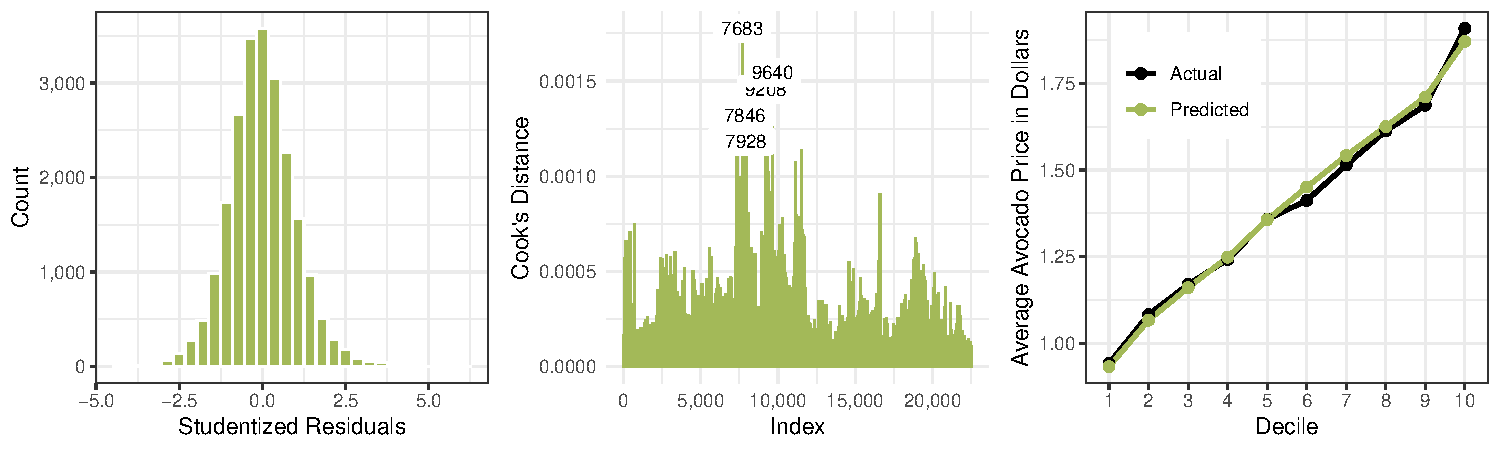
\includegraphics[width=\maxwidth]{figure/unnamed-chunk-4-1} 

\caption{1 (Left): Lift chart of empirical (black) and indicated (blue) penetration rate sorted from smallest to largest and assinged by decile and 2 (Right): Cook's Distance plot with labeled outlier observations.}
\label{model_plot_1}
\end{center} 
\end{figure}

\noindent Checking the quality of the model is one of the most important step in a data analysis. First, multicolineary would not be an issue in this analysis since VIF scores are smaller than 2 for each variable. Secondly, Figure~\ref{model_plot_1}.2 shows the Cook's distance of each observation point. A few observations did not meet the cutoff point of 0.02 including rows 4, 7, 87, 121, 157, 196, 239, 254, 267, 272, 289, 307, and 365. These points influence all fitted values. In other words, these subjects have huge impact on the chances of getting penetrated of prostate capsule.     
\hfill \break

\noindent The student residuals are also very important to validate while accessing the quality of the model. Figure~\ref{model_plot_2}.1 portrays a residual plot of the model. The plots is color coded by two section, one for underestimate points and one for over estimate subjects. The number of overestimte values and overestimate values are approximately the same which constructed a mean value for resudials is approximately 0 or -0.07 to be exact. Furthermore, there are no pattern to be detected in the residuals consistent with constant variance. Most residuals are between -2 and 2 which is ideal for all residuals. However, there are a few points that clearly have large residuals including rows 87, 239, and 289. This indicates that these three subjects are outliers.         

\begin{figure}[h!] 
\begin{center}

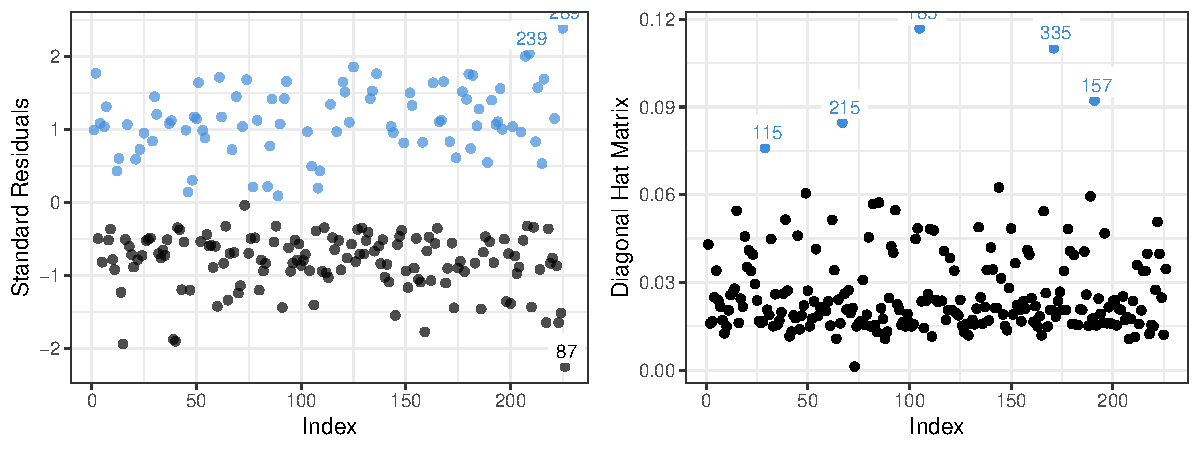
\includegraphics[width=\maxwidth]{figure/unnamed-chunk-5-1} 

\caption{1 (Left): Studendized residuals plot with blue color are positive residuals (overestimate values) and black are negatie residuals (underestimate values), and 2 (Right): Diagonal hat matrix plot with influential points in colored in blue.}
\label{model_plot_2}
\end{center} 
\end{figure}

\noindent Lastly, large hat values show potential outlying observation with respect to each predictors. As seen in Figure~\ref{model_plot_2}, rows 115, 215, 185, and 335. These subjects potentially have really high/low values consisted in one or more of their predictors. To further access the outliers and influential points, Table~A\ref{outlier_obs} was constructed to show the details of each observation that were detected as outliers or influential points. Most subjects noticibly have really high PSA scores compare to the mean PSA scores of 15.26. However, all subjects were decided to be kept in the model since there are no valid reasons to remove them from the model.       
\hfill \break

\noindent After finishing model development and validation, the model is ready for interpretation. All interpretaion values used in this section are from Table~\ref{reg_summary_final}. The results of digital exam has great impact on penetration. For instant, a patient with a unilobar nodule (left) would be 2.28 times or 128\% riskier than a patient without a nodule. A person with a unilobar nodule (right) would be 3.69 times or 269\% more likely to have their tumor penetrated with prostate capsule. Lastly, a person with bilobar nodule would be more likely to be diagnosed with prostate cancer 3.60 times compared to patients with no nodule. In addition, a patient as PSA scores increases by 1 mg/ml, on average, the patient will have 4\% increase in the risk of having a prostate cancer. Last but not least, having a low Gleason score would decrease the chances of having cancer since an increase of 1-unit in Gleason score would cause the patient to be 2.33 times riskier.   
\hfill \break

\noindent\textbf{\underline{Conclusion}}: Generally, there are protocols for doctors and nurses to follow when it comes to important diagnosis like prostate cancer. Manually, it is quite difficult to avoid human error when providing a dignostic to a patient. With this model, health professionals can be able to minimize predicting errors and generate the likelihood of a men getting prostate cancer efficiently. The three main factors that change the chance of a tumor have pentrated of prostate capsule are the results of digital rectal exam, PSA scores, and total Gleason scores. Penetration rate are likely to inscrease as the results of digital rectal exam are in a critical nodule, PSA are higher, and total Gleason scores are larger. On the other hand, having no nodule in the results of digital rectal exam, low PSA scores, and low Gleason scores would cause the likelihood of penetration to be very low. This leads to lower risk of having prostate cancer. With an AUC of 0.82 and accuracy of 0.77, we can consider this model to be the best model that can provide the likelihood of penetration rate in men. There are many limiations for this models. First, the sample size in this dataset is relatively small. The subset of this small sample size could cause the results to be not as accurate as the full dataset. If we have access to the full dataset from the Ohio State University Comprehensive Cancer Center, then our results might be different. In addition, there were only 6 preditors provided to use in the model. If there is more variables, the model could provide better results. For example, we can consider genetic could also be a factor that cause the risk of having prostate cancer in the family of the patient to improve the current model.          
\hfill \break

\clearpage
\newpage
\noindent \Large{{\bf Appendix A: Supplemental Tables}}

\begin{center}

% Table created by stargazer v.5.2.2 by Marek Hlavac, Harvard University. E-mail: hlavac at fas.harvard.edu
% Date and time: Sun, Nov 08, 2020 - 1:09:51 PM
\begin{table}[H] \centering 
  \caption{Summary Statistics for all independent features} 
  \label{descrips} 
\begin{tabular}{@{\extracolsep{5pt}}lccccccc} 
\\[-1.8ex]\hline 
\hline \\[-1.8ex] 
Statistic & \multicolumn{1}{c}{N} & \multicolumn{1}{c}{Mean} & \multicolumn{1}{c}{St. Dev.} & \multicolumn{1}{c}{Min} & \multicolumn{1}{c}{Pctl(25)} & \multicolumn{1}{c}{Pctl(75)} & \multicolumn{1}{c}{Max} \\ 
\hline \\[-1.8ex] 
age & 377 & 66.066 & 6.425 & 47 & 62 & 71 & 79 \\ 
psa & 377 & 15.256 & 19.869 & 0.300 & 5.000 & 16.800 & 139.700 \\ 
gleason & 377 & 6.379 & 1.092 & 0 & 6 & 7 & 9 \\ 
\hline \\[-1.8ex] 
\end{tabular} 
\end{table} 

\end{center} 

\begin{center}
% latex table generated in R 3.6.2 by xtable 1.8-4 package
% Sun Nov 08 13:09:51 2020
\begin{table}[ht]
\centering
\begin{tabular}{rrrrlrr}
  \hline
 & random\_partition & nrow\_train & nrow\_test & features & AIC & auc \\ 
  \hline
1 & 0.900 &  339 &   38 & dpros,psa,gleason,dcaps & 298.077 & 0.822 \\ 
  2 & 0.800 &  301 &   76 & dpros,psa,gleason,dcaps & 278.940 & 0.820 \\ 
  3 & 0.600 &  226 &  151 & dpros,psa,gleason & 241.799 & 0.819 \\ 
  4 & 0.700 &  263 &  114 & dpros,psa,gleason & 260.832 & 0.818 \\ 
  5 & 0.600 &  226 &  151 & dpros,psa,gleason,dcaps & 240.567 & 0.818 \\ 
  6 & 0.700 &  263 &  114 & dpros,psa,gleason,dcaps & 258.675 & 0.815 \\ 
  7 & 0.900 &  339 &   38 & dpros,psa,gleason & 297.050 & 0.812 \\ 
  8 & 0.800 &  301 &   76 & dpros,psa,gleason & 277.654 & 0.809 \\ 
  9 & 0.600 &  226 &  151 & psa,gleason,dcaps & 251.167 & 0.805 \\ 
  10 & 0.900 &  339 &   38 & dpros,gleason & 301.355 & 0.805 \\ 
   \hline
\end{tabular}
\caption{Iteration log of model bootstraping process. Showing the top 10 models that have the highest AUC scores. The columns represent random partition for train set, number of rows in the training data, number of rows in the testing data, predictors, AIC scores, and AUC scores, respectively from left to right.} 
\label{reg_bootstrap}
\end{table}

\end{center}

\begin{center}
% latex table generated in R 3.6.2 by xtable 1.8-4 package
% Sun Nov 08 13:09:51 2020
\begin{table}[ht]
\centering
\begin{tabular}{rrrrr}
  \hline
 & Estimate & Std. Error & z value & Pr($>$$|$z$|$) \\ 
  \hline
(Intercept) & -9.7465 & 3.8714 & -2.52 & 0.0118 \\ 
  dpros2 & 1.7503 & 4.1518 & 0.42 & 0.6733 \\ 
  dpros3 & 2.9024 & 4.2654 & 0.68 & 0.4962 \\ 
  dpros4 & 4.8459 & 4.7046 & 1.03 & 0.3030 \\ 
  psa & 0.2090 & 0.1227 & 1.70 & 0.0886 \\ 
  gleason & 1.0748 & 0.6161 & 1.74 & 0.0811 \\ 
  dpros2:psa & -0.0986 & 0.0638 & -1.55 & 0.1221 \\ 
  dpros3:psa & -0.1225 & 0.0801 & -1.53 & 0.1260 \\ 
  dpros4:psa & -0.0601 & 0.0699 & -0.86 & 0.3902 \\ 
  dpros2:gleason & 0.0468 & 0.6584 & 0.07 & 0.9434 \\ 
  dpros3:gleason & -0.0354 & 0.6803 & -0.05 & 0.9585 \\ 
  dpros4:gleason & -0.4452 & 0.7431 & -0.60 & 0.5491 \\ 
  psa:gleason & -0.0130 & 0.0168 & -0.77 & 0.4396 \\ 
   \hline
\end{tabular}
\caption{Summary regresson of the final model with all combination of interaction terms. The columns represent the variables, coefficient estimated values, standard error, test statistics, and signficant p-values, respectively from left to right.} 
\label{reg_summary_int}
\end{table}

\end{center}

\begin{center}
% latex table generated in R 3.6.2 by xtable 1.8-4 package
% Sun Nov 08 13:09:51 2020
\begin{table}[ht]
\centering
\begin{tabular}{rrlrrl}
  \hline
 & capsule & dpros & psa & gleason & rownames \\ 
  \hline
1 &   0 & 2 & 51.20 &   7 & 4 \\ 
  2 &   0 & 4 & 31.90 &   7 & 7 \\ 
  3 &   0 & 4 & 17.10 &   9 & 87 \\ 
  4 &   1 & 4 & 45.30 &   6 & 115 \\ 
  5 &   0 & 4 & 25.20 &   7 & 121 \\ 
  6 &   1 & 1 & 44.40 &   6 & 157 \\ 
  7 &   1 & 1 & 85.40 &   7 & 185 \\ 
  8 &   1 & 3 & 17.70 &   5 & 196 \\ 
  9 &   1 & 4 & 53.90 &   6 & 215 \\ 
  10 &   1 & 1 & 6.70 &   6 & 239 \\ 
  11 &   0 & 4 & 25.10 &   7 & 254 \\ 
  12 &   1 & 4 & 18.70 &   5 & 267 \\ 
  13 &   1 & 1 & 8.90 &   6 & 272 \\ 
  14 &   1 & 1 & 6.80 &   5 & 289 \\ 
  15 &   0 & 3 & 18.10 &   8 & 307 \\ 
  16 &   1 & 2 & 58.00 &   6 & 335 \\ 
  17 &   0 & 2 & 48.00 &   7 & 365 \\ 
   \hline
\end{tabular}
\caption{Table of all potential outlier and influential values. The columns represent the tumor penetration of prostatic capsule, results of digital rectal exam, PSA scores, total Gleason scores, and row number of each subject, respectively from left to right.} 
\label{outlier_obs}
\end{table}

\end{center}


\clearpage
\newpage
\noindent \Large{{\bf Appendix B: R Code}}
\lstinputlisting[language=R, caption = Appendix of Code]{R/dar2-codes.R}


\end{document}






